\chapter{Reference Distance}

This chapter describes the result of the distance measurements for the defined reference data. All calculations and graphs shown in this chapter are produced in the Jupyter Notebook 
\newline \path{DistanceReferenceMeasurement.ipynb}.

\section{One Hour Reference Time Series}

Due to the rough granularity of one hour both distance measures produce the same result. This is also visualised by the straight diagonal red line in figure \ref{fig:ref_dtw_dist_one_h_granularity}.

\subsection{Euclidean Distance}

The Euclidean Distance between the \ac{hr} time series is: \textbf{0.198673}


The Euclidean Distance between the \ac{rr} time series is: \textbf{0.316962}


The Euclidean Distance between the \ac{mss} time series is: \textbf{0.285505}


\subsection{DTW}

The distance using \ac{dtw} between the \acp{hr} values is: \textbf{0.198673}


The distance using \ac{dtw} between the \acp{rr} values is: \textbf{0.316962}


The distance using \ac{dtw} between the \acp{mss} values is: \textbf{0.285505}



\begin{figure}[h!]
	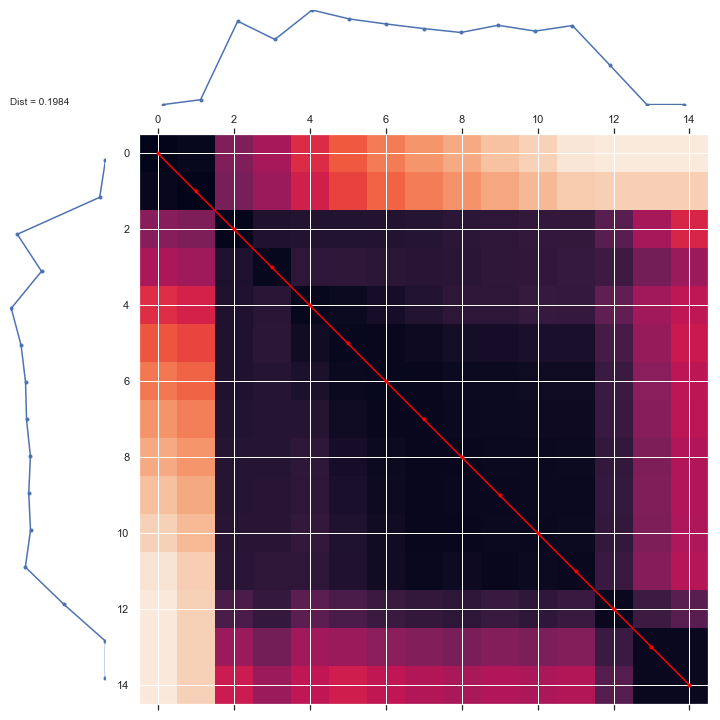
\includegraphics[width=1\textwidth]{ref_1hour_hr_dtw.png}
	\caption{DTW visualisation (HR, 1h granularity)}
	\label{fig:ref_dtw_dist_one_h_granularity}
\end{figure}




\clearpage
\section{30 Minutes Reference Time Series}

Due to the rough granularity of 30min there is no big difference between the Euclidean and \ac{dtw} method. As one can see in figure \ref{fig:ref_dtw_dist_30_min_granularity}, the warping path is still almost a straight diagonal line.

\subsection{Euclidean Distance}

The Euclidean Distance between the \ac{hr} time series is: \textbf{0.369976}


The Euclidean Distance between the \ac{rr} time series is: \textbf{0.775827}



The Euclidean Distance between the \ac{mss} time series is: \textbf{0.508129}



\subsection{DTW}

The distance using \ac{dtw} between the \acp{hr} values is: \textbf{0.327602}


The distance using \ac{dtw} between the \acp{rr} values is: \textbf{0.775718}


The distance using \ac{dtw} between the \acp{mss} values is: \textbf{0.508129}



\begin{figure}[h!]
	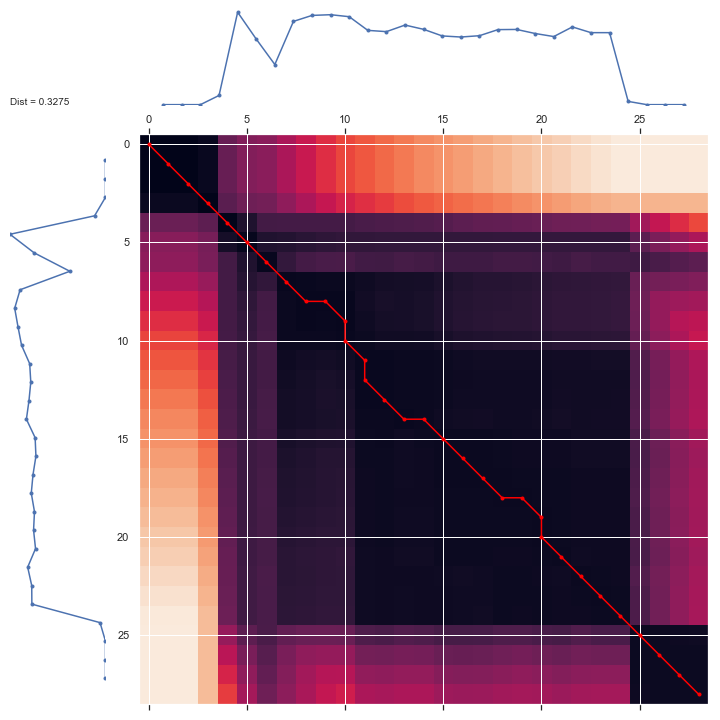
\includegraphics[width=0.6\textwidth]{ref_30min_hr_dtw.png}
	\caption{DTW visualisation (HR, 30min granularity)}
	\label{fig:ref_dtw_dist_30_min_granularity}
\end{figure}


\clearpage
\section{Five Minutes Reference Time Series}

Due to the finer granularity there will bigger differences between the two time series in terms of noise. Thus, the Euclidean and \ac{dtw} distances increase. Therefore, \ac{dtw} have a greater impact than in the previous observations as figure \ref{fig:ref_dtw_dist_5_min_granularity} indicates.

\subsection{Euclidean Distance}

The Euclidean Distance between the \ac{hr} time series is: \textbf{2.095002}


The Euclidean Distance between the \ac{rr} time series is: \textbf{3.644268}


The Euclidean Distance between the \ac{mss} time series is: \textbf{1.993386}


\subsection{DTW}

The distance using \ac{dtw} between the \acp{hr} values is: \textbf{1.600346}


The distance using \ac{dtw} between the \acp{rr} values is: \textbf{2.585769}


The distance using \ac{dtw} between the \acp{mss} values is: \textbf{1.674696}



\begin{figure}[h!]
	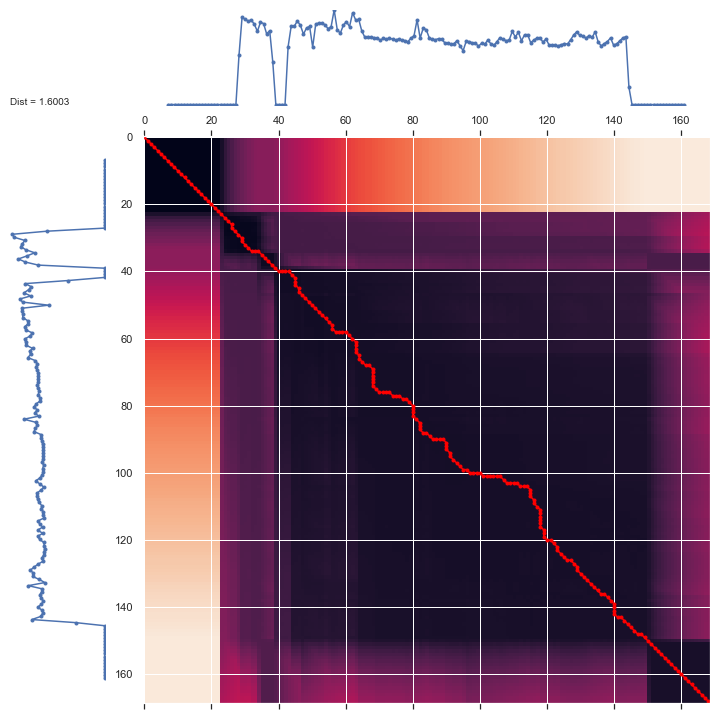
\includegraphics[width=0.6\textwidth]{ref_5min_hr_dtw.png}
	\caption{DTW visualisation (HR, 5min granularity)}
	\label{fig:ref_dtw_dist_5_min_granularity}
\end{figure}






\clearpage
\section{One Minute Reference Time Series}

Now, for the granularity of one minute the \ac{dtw} distance is almost only half of the euclidean distance.

\subsection{Euclidean Distance}

The Euclidean Distance between the \ac{hr} time series is: \textbf{7.455447}


The Euclidean Distance between the \ac{rr} time series is: \textbf{10.56793}


The Euclidean Distance between the \ac{mss} time series is: \textbf{11.502093}



\subsection{DTW}

The distance using \ac{dtw} between the \acp{hr} values is: \textbf{3.888863}


The distance using \ac{dtw} between the \acp{rr} values is: \textbf{5.810633}


The distance using \ac{dtw} between the \acp{mss} values is: \textbf{5.575821}


\begin{figure}[h!]
	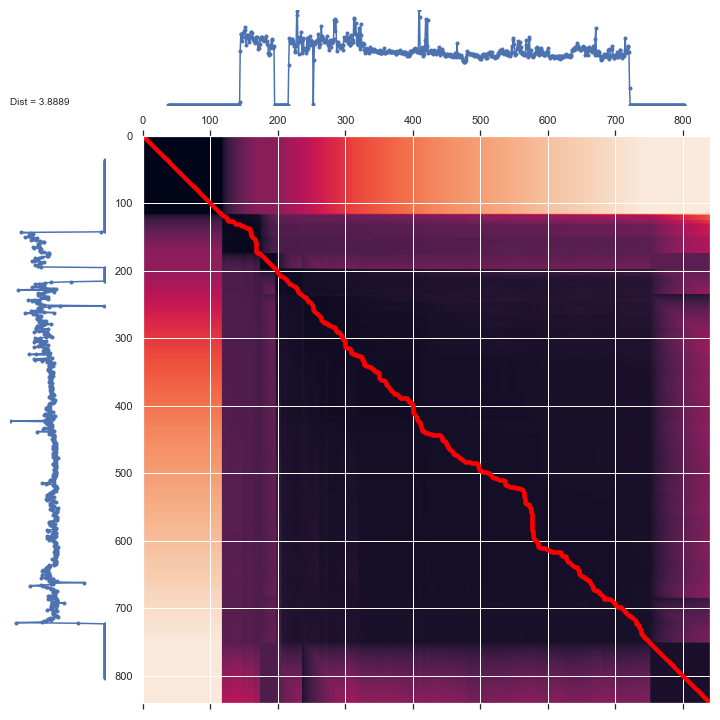
\includegraphics[width=0.6\textwidth]{ref_1min_hr_dtw.png}
	\caption{DTW visualisation (HR, 1min granularity)}
	\label{fig:ref_dtw_dist_1_min_granularity}
\end{figure}


\clearpage
\section{Conclusion}

Table \ref{tab:ref_dist_compare} provides an overview over the calculated reference distances. One can clearly see that the finer the granularity gets the larger the distances will become. Similarly the ratios of the euclidean distance and the \ac{dtw} distance increase.

\begin{table}[h!]
\centering
\resizebox{\textwidth}{!}{
	\begin{tabular}{|c||c|c||c|c||c|c|}\hline
		{} &  
		\multicolumn{2}{|c||}{\textbf{\ac{hr}}} & 
		\multicolumn{2}{|c||}{\textbf{\ac{rr}}} & 
		\multicolumn{2}{|c|}{\textbf{\ac{mss}}}\\
		\hline
		% specify table head
		\bfseries Granularity & 
		\bfseries Euclidean &
		\bfseries \ac{dtw} &
		\bfseries Euclidean &
		\bfseries \ac{dtw} &
		\bfseries Euclidean &
		\bfseries \ac{dtw} \\
		\hline\hline
		1 Hour & 0.198673 & 0.198673 & 0.316962 & 0.316962 & 0.285505 & 0.285505 \\
		\hline
		30 Min & 0.369976 & 0.327602 & 0.775827 & 0.775718 & 0.508129 & 0.508129 \\
		\hline
		5 Min & 2.095002 & 1.600346 & 3.644268 & 2.585769 & 1.993386 & 1.674695 \\
		\hline
		1 Min & 7.455447 & 3.888863 & 10.56793 & 5.810633 & 11.502094 & 5.575821 \\
		\hline

	\end{tabular}
}
\caption{Reference Distances Comperation}
\label{tab:ref_dist_compare}
\end{table}

Whenever a distance between two time series will be calculated during this project, it can be compared to these reference distances in order to determine "how good/bad" the distance actually is.





